% This template has been tested with LLNCS DOCUMENT CLASS -- version 2.20 (24-JUN-2015)

%"runningheads" enables:
%  - page number on page 2 onwards
%  - title/authors on even/odd pages
%This is good for other readers to enable proper archiving among other papers and pointing to content.
%Even if the title page states the title, when printed and stored in a folder, when blindly opening the folder, one could hit not the title page, but an arbitrary page. Therefore, it is good to have title printed on the pages, too.
\documentclass[runningheads,a4paper]{llncs}[2015/06/24]

%Even though `american`, `english` and `USenglish` are synonyms for babel package (according to https://tex.stackexchange.com/questions/12775/babel-english-american-usenglish), the llncs document class is prepared to avoid the overriding of certain names (such as "Abstract." -> "Abstract" or "Fig." -> "Figure") when using `english`, but not when using the other 2.
\usepackage[english]{babel}

%better font, similar to the default springer font
%cfr-lm is preferred over lmodern. Reasoning at http://tex.stackexchange.com/a/247543/9075
\usepackage[%
rm={oldstyle=false,proportional=true},%
sf={oldstyle=false,proportional=true},%
tt={oldstyle=false,proportional=true,variable=true},%
qt=false%
]{cfr-lm}
%
%if more space is needed, exchange cfr-lm by mathptmx
%\usepackage{mathptmx}

\usepackage{graphicx}

%% If you need packages for other papers,
%% START COPYING HERE

%extended enumerate, such as \begin{compactenum}
\usepackage{paralist}
\usepackage{multirow}

\usepackage{amsmath}
%put figures inside a text
%\usepackage{picins}
%use
%\piccaptioninside
%\piccaption{...}
%\parpic[r]{\includegraphics ...}
%Text...

%Sorts the citations in the brackets
%It also allows \cite{refa, refb}. Otherwise, the document does not compile.
%  Error message: "White space in argument"
\usepackage{cite}

\usepackage[T1]{fontenc}
\usepackage{cmap}

%for demonstration purposes only
\usepackage[math]{blindtext}

%for easy quotations: \enquote{text}
\usepackage{csquotes}

%enable margin kerning
\usepackage{microtype}

%tweak \url{...}
\usepackage{url}
\urlstyle{same}
%improve wrapping of URLs - hint by http://tex.stackexchange.com/a/10419/9075
\makeatletter
\g@addto@macro{\UrlBreaks}{\UrlOrds}
\makeatother
%nicer // - solution by http://tex.stackexchange.com/a/98470/9075
%DO NOT ACTIVATE -> prevents line breaks
%\makeatletter
%\def\Url@twoslashes{\mathchar`\/\@ifnextchar/{\kern-.2em}{}}
%\g@addto@macro\UrlSpecials{\do\/{\Url@twoslashes}}
%\makeatother

%diagonal lines in a table - http://tex.stackexchange.com/questions/17745/diagonal-lines-in-table-cell
%slashbox is not available in texlive (due to licensing) and also gives bad results. This, we use diagbox
%\usepackage{diagbox}

%required for pdfcomment later
\usepackage{xcolor}

% new packages BEFORE hyperref
% See also http://tex.stackexchange.com/questions/1863/which-packages-should-be-loaded-after-hyperref-instead-of-before

%enable hyperref without colors and without bookmarks
\usepackage[
%   pdfauthor={},
%   pdfsubject={},
%   pdftitle={},
%   pdfkeywords={},
   bookmarks=false,
   colorlinks=true,
   allcolors=black,
   pdfstartview=Fit,
   breaklinks=true,
]{hyperref}
%enables correct jumping to figures when referencing
\usepackage[all]{hypcap}

%enable nice comments
\usepackage{pdfcomment}
\newcommand{\commentontext}[2]{\colorbox{yellow!60}{#1}\pdfcomment[color={0.234 0.867 0.211},hoffset=-6pt,voffset=10pt,opacity=0.5]{#2}}
\newcommand{\commentatside}[1]{\pdfcomment[color={0.045 0.278 0.643},icon=Note]{#1}}

%compatibality with packages todo, easy-todo, todonotes
\newcommand{\todo}[1]{\commentatside{#1}}
%compatiblity with package fixmetodonotes
\newcommand{\TODO}[1]{\commentatside{#1}}

%enable \cref{...} and \Cref{...} instead of \ref: Type of reference included in the link
\usepackage[capitalise,nameinlink]{cleveref}
%Nice formats for \cref
\crefname{section}{Sect.}{Sect.}
\Crefname{section}{Section}{Sections}

\usepackage{xspace}
%\newcommand{\eg}{e.\,g.\xspace}
%\newcommand{\ie}{i.\,e.\xspace}
\newcommand{\eg}{e.\,g.,\ }
\newcommand{\ie}{i.\,e.,\ }

%introduce \powerset - hint by http://matheplanet.com/matheplanet/nuke/html/viewtopic.php?topic=136492&post_id=997377
\DeclareFontFamily{U}{MnSymbolC}{}
\DeclareSymbolFont{MnSyC}{U}{MnSymbolC}{m}{n}
\DeclareFontShape{U}{MnSymbolC}{m}{n}{
    <-6>  MnSymbolC5
   <6-7>  MnSymbolC6
   <7-8>  MnSymbolC7
   <8-9>  MnSymbolC8
   <9-10> MnSymbolC9
  <10-12> MnSymbolC10
  <12->   MnSymbolC12%
}{}
\DeclareMathSymbol{\powerset}{\mathord}{MnSyC}{180}

% correct bad hyphenation here
\hyphenation{op-tical net-works semi-conduc-tor}

%% END COPYING HERE

\begin{document}

\title{Implementation of a Brute Force Attack on the A5/1 Keystream Generator
in a GPU-based Volunteer Computing Project}
\titlerunning{Brute Force Attack on A5/1}

%Single insitute
\author{Vadim Bulavintsev \and Alexander Semenov \and Oleg Zaikin}
\authorrunning{Vadim Bulavintsev et al.}
\institute{Matrosov Institute for System Dynamics and Control Theory of
Siberian Branch of Russian Academy of Sciences, Irkutsk, Russia
\email{v.g.bulavintsev@gmail.com, biclop.rambler@yandex.ru, zaikin.icc@gmail.com}}
			
\maketitle

\begin{abstract}
We present an advanced brute force attack on the A5/1 keystream generator,
that is still widely used in modern GSM networks. We use a
well-known idea introduced by R. Anderson more than 20 years ago
to greatly reduce the search space. The main contribution of
the present paper is the implementation of Anderson's attack on a GPU platform
with bit-slice technique. The preliminary estimates of the
attack's speed showed that, with the use of GPUs processing power, 
the attack could be performed in the real time on a modern computer cluster or in a volunteer computing
project. To verify our estimates with the use of the BOINC technology 
we launched a volunteer computing project and executed our variant of Anderson's attack within it. 
As a result, 10 A5/1 cryptanalysis problems were solved in 7 days in the project. 
The results presented in this work provide yet another proof of A5/1's cryptographic 
weakness which shows that this generator is totally unsuitable for transmission of any kind of sensitive data
through modern GSM networks.
\end{abstract}

\begin{keywords}
keystream generator, A5/1, cryptanalysis, brute force attack, GPU, volunteer computing, BOINC
\end{keywords}

\section{Introduction}
\label{sec:intro}

The A5/1 keystream generator has a key length of 64 bits. It is used
to encrypt voice and SMS traffic in 2nd generation (2G) GSM networks. 3rd
generation (3G) GSM networks allows to use 2G communication protocol in order to maintain the backward
compatibility.

A5/1 is one of the most publicly recognized cryptographic
algorithms, along with RSA and DES, its discussion reaching far beyond the
borders of cryptographers community. For example, article
\cite{Timberg2013} publicly discusses NSA's ability to efficiently decrypt A5/1.
In the present paper we will not touch on the details of A5/1's development history
and the reasons of its rise as the most popular cryptographic algorithm for mobile communication. 

Among all the different methods of A5/1 cryptanalysis we distinguish those
which were implemented in practice and allowed to reliably perform the
cryptanalysis procedure for the non-weakened variant of the algorithm. Apparently,
the first such attack was performed in 2008 with the help of the special
FPGA-based computational platform COPACOBANA \cite{DBLP:conf/ches/GendrullisNR08}. In 2009 distributed
algorithms for Boolean satisfiability problem (SAT) were used to solve several A5/1
cryptanalysis instances in BNB-Grid\cite{Posypkin2009}. These results were further improved in 2011 \cite{DBLP:conf/pact/SemenovZBP11}. By the end of 2009 the \textit{A5/1 Cracking Project} had published rainbow tables
\cite{Nohl2010} for A5/1. Provided with 8 bursts (912 bits) of keystream these
tables allowed to find the secret key in less than a minute with more than 85\%
probability. Despite the huge (over 2 Tb) size, to this day these rainbow tables
provide the most practical method of A5/1 cryptanalysis. Its main shortcoming
is that the probability of success is significantly less than 100\%. 

Meanwhile, the growth of computational power of GPUs and FPGAs made it possible to put into practice the attack,
which was described by R. Anderson in 1994 \cite{Anderson1994}. This attack is based on reduction of the search space from $2^{64}$ to $2^{53}$.  As was mentioned earlier, FPGA-based variant of Anderson's attack was already performed in 2008 in the COPACOBANA project. So, the primary goal of our work is to demonstrate the viability of
GPU-based variant of the attack. Let us note that GPUs are much easier to
operate than FPGAs, and the former belong to the class of consumer-grade
devices and could be found in any modern PC, while the latter belong to the
class of specialized equipment.  With the usage of the BOINC software platform
\cite{Anderson:2004:BSP:1032646.1033223}, these qualities of GPUs allowed us to implement the attack in
the form of a volunteer computing project using idle computational
capabilities of the project members home PCs.  Our estimates of the attack's speed
were based on our previous work\cite{BulavintsevS2016}.

Let us make a brief outline of the article's contents. In \Cref{sec:alg} we
describe the A5/1 algorithm along with some advanced brute force attacks on it.
\Cref{sec:bitslc} introduces bit-slicing technique and goes through important
details of implementing Anderson's attack. \Cref{sec:boinc}
provides a look into the internal organization of the volunteer project which was launched by us to perform the attack. \Cref{sec:related} contains the retrospective of A5/1 cryptanalysis works related to our study.

%%%%%%%%%%%%%%%%%%%%%%%%%%%%%%%%%%%%%%%%%%%%%%%%%%%%%%%%%%%%%%%%%%%%%%%%%%%%%%%
\section{A5/1 keystream generator and some attacks on it}
\label{sec:alg}
%%%%%%%%%%%%%%%%%%%%%%%%%%%%%%%%%%%%%%%%%%%%%%%%%%%%%%%%%%%%%%%%%%%%%%%%%%%%%%%

The A5/1 keystream generator consists of 3 linear feedback shift registers (\mbox{LFSRs} \cite{Menezes:1996:HAC:548089}), 
defined by the following primitive polynomials:

\begin{gather*} 
	LFSR1: X^{19}+X^{18}+X^{17}+X^{14}+1;\\
	LFSR2: X^{22}+X^{28}+1;\\
	LFSR3: X^{23}+X^{22}+X^{21}+X^{8}+1, LFSR3.
\end{gather*}

The illustration of the A5/1 generator's scheme can be seen at
\cref{fig:a51gen}.

\begin{figure}
	\centering
	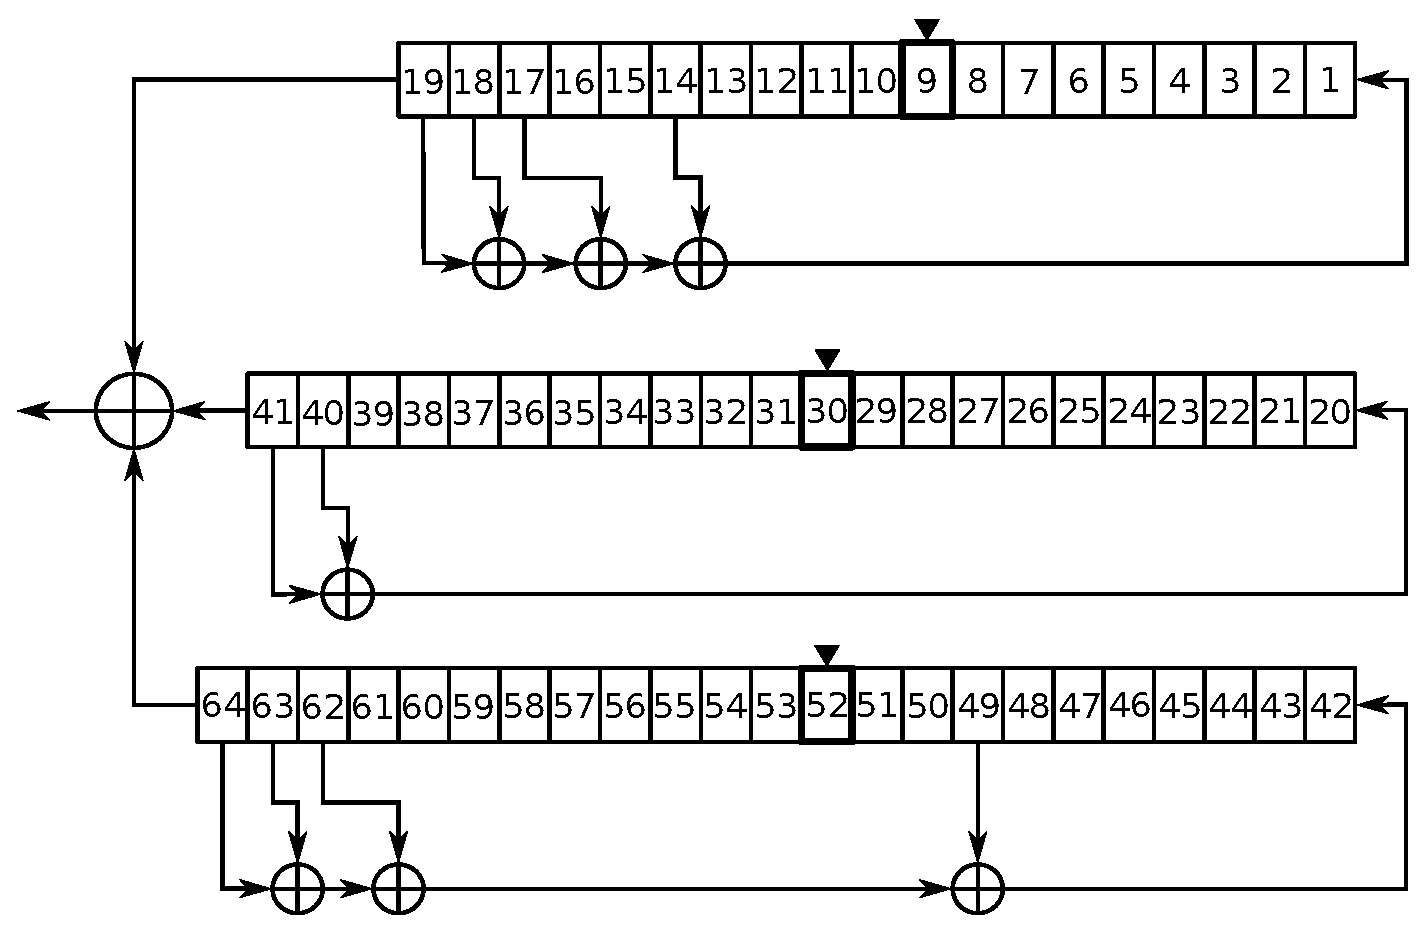
\includegraphics[width=8cm]{./a51.eps} 
	\caption{The A5/1 generator scheme} 
	\label{fig:a51gen} 
\end{figure}

The outputs of LFSRs are mixed by linear function, that provides the best
correlation immunity. Non-linearity of the cryptanalysis equations is achieved by clocking
the registers asynchronously --- for each clocking of the generator any LFSR 
can be shifted or it can retain its current state.
LFSR with index $j \in \{1,2,3\}$ is shifted if the following Boolean
function $\chi_j$ takes the value of 1:

\begin {gather*}
\chi_j = (b_j \equiv majority(b_1,b_2,b_3)); 
\\majority(A,B,C)=(A \wedge B) \vee (A \wedge C) \vee (B \vee C).
\end{gather*}

Here $b_1,b_2,b_3$ denote clocking bits marked at \cref{fig:a51gen} by black
wedges. Conversely, if at some moment $\chi_j=0$, LFSR$j$ is not shifted (it
remains in its last state).

Generator A5/1 is used in the GSM protocol for high-speed encryption of large
volumes of information. The whole process is splitted into \textit{sessions}. Each session uses its own session key, and has length about 3.5 hours. We will not touch on the topic of specialized protocols used in GSM networks to
build and transfer the session key.

Along the message data, GSM protocol sends error correction data for the
message. The combination of the message data with the error correction data constitutes a 456 bits
long \textit{frame}, which is splitted into 4 \textit{bursts} of 114 bits. The
bursts are then encrypted and sent over the air. To encrypt a burst the A5/1
generator is initialized with the 64-bit \textit{local key}, that is built using
session key and a natural number called \textit{frame number} (FN). After the
encryption of one burst is complete, FN is increased by 1. When
FN overflows, the session ends and a new session is initialized.

If the message length is less than 23 bytes, the message is filled with
fixed pattern padding to 23 bytes. During the call, some GSM technical messages have fixed length and are always padded. As padding is always the same, and it is encrypted by some local key, we get a typical plain text attack
scenario \cite{Menezes:1996:HAC:548089}. Indeed, the padding plays the role of the
known plaintext, allowing the attacker to get the corresponding keystream
fragment. This vulnerability allows the attacker to obtain no less than two frames
(912 bits) of the keystream. It was demonstrated in \cite{Nohl2010,GlendrangeHH2010} that the
knowledge of even one local key and FN is enough to efficiently restore the
session key, which makes the decryption of the whole session possible.

The described vulnerability of the GSM protocol allows to build some successful
attacks on it, based on the idea of ``advanced brute force''. In particular, the
large-scale preprocessing made it possible to create the rainbow tables,
which, provided 8 bursts of keystream, allows to determine the session key in less than a minute with $>85\%$ probability. The tables take about 2 Tb of disk space. This attack is presented in detail in \cite{Nohl2010},
and still stands among the most practical ones. Further, we will focus on the
idea of an attack that was suggested by Ross Anderson in 1994 in a small essay
on the A5/1 cryptographic resistance \cite{Anderson1994}. Next we describe the
essence of Anderson's attack.

\begin{figure}
	\centering
	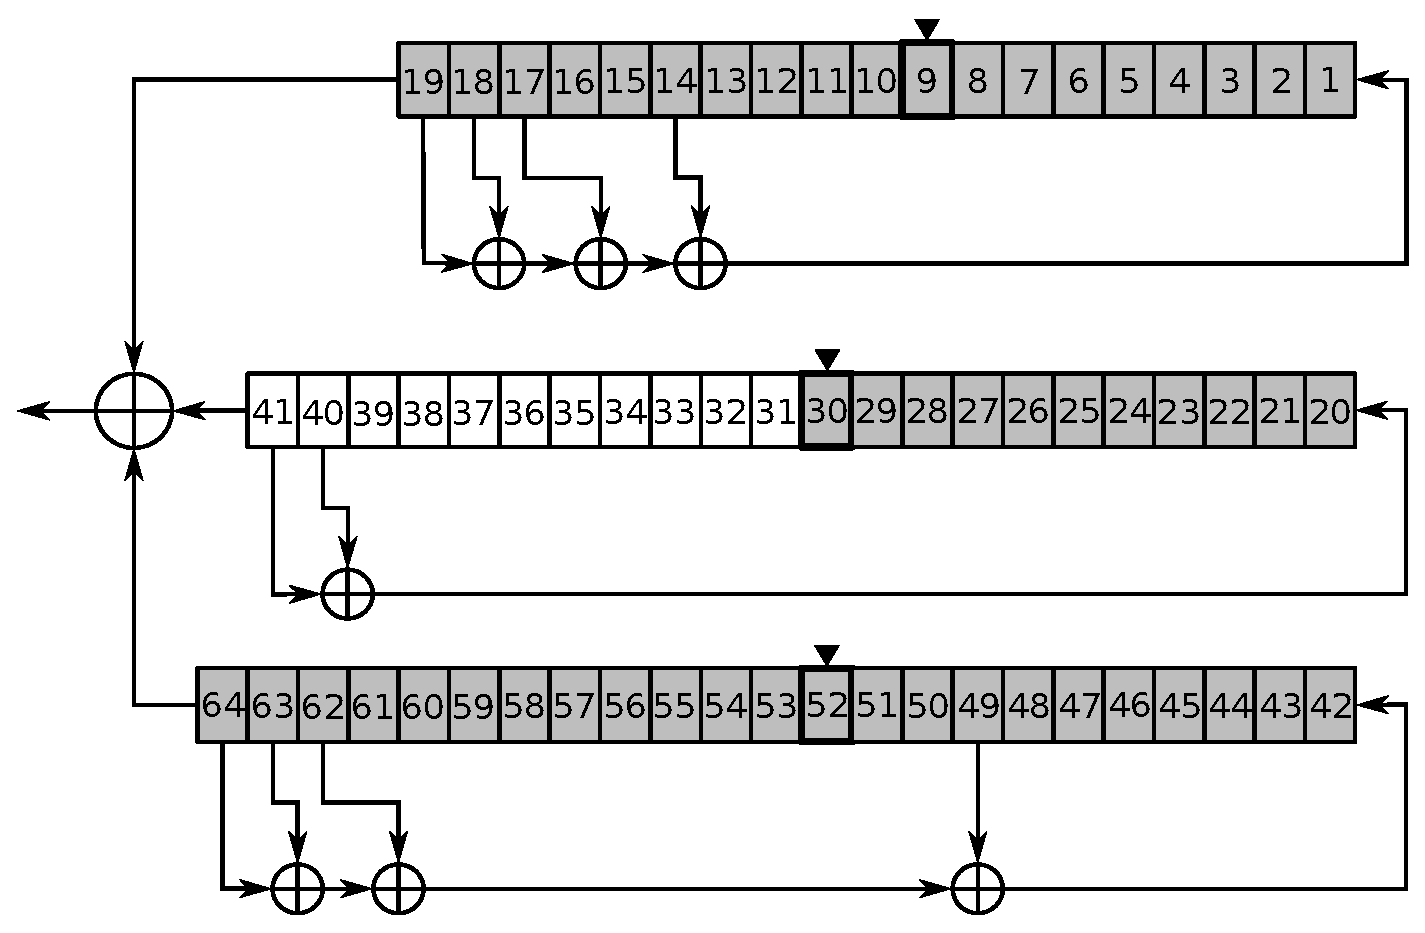
\includegraphics[width=8cm]{./a51and.eps} 
	\caption{The set of guessing bits used in Anderson's attack (greyed out).}
	\label{fig:a51and}
\end{figure}

Anderson's attack is a typical example of a \textit{guess and determine attack} (see, for example,
\cite{Bard:2009:AC:1618541}). Suppose that we know the bits filling LFSR1 and LFSR3, and
bits of LFSR2 from the beginning of the register to the clocking bit
(bits 31 to 41, see \cref{fig:a51and}). Next, suppose that we know 64 bits of the
keystream. It was shown by R. Anderson, that 11 unknown bits of LFSR2
can be figured out without any additional guesses. This is possible because the following data is known:

\begin{itemize}
\item the clocking bits (so, the clocking schedule for the next 11 shifts of LFSR2 is also known); 
\item 2 out of 3 LFSRs output bits, which are taken as input for the XOR operation; 
\item the result of the XOR operation (from the keystream). 
\end{itemize}

Therefore, one can efficiently derive the unknown bits of LFSR2 one by one, by clocking the
generator and applying XOR operation to corresponding keystream bits and output
bits of LFSR1 and LFSR3.

The considered algorithm, that is used to determine the unknown 11 bits of LFSR2,
makes it possible to mount a brute force attack on the A5/1 generator over the search space with the size of $2^{53}$. The simplicity of the algorithm provides an opportunity to implement it on a specialized
computational architecture. One such implementation was built with FPGAs by
authors of \cite{DBLP:conf/ches/GendrullisNR08}. In the following sections we describe our
implementation of this attack for modern GPUs.

\section{Implementation of Anderson's Attack in bit-slicing technique}
\label{sec:bitslc}

The efficiency of a brute force attack is defined by two parameters: the speed
of checking of the key candidates and the size of the search space. R. Anderson's idea described above gives us the search space with the size of $2^{53}$. 
Instead of using the ``naive'' implementation of the A5/1 generator, to speed up the key candidates checking procedure one can opt to use more
sophisticated alternatives. We evaluated the performance of two different fast
implementations of A5/1 generator in \cite{BulavintsevS2016}. The first one was based
on an idea of precomputation of the states of LFSR1-3, and
keeping these states in PC's memory. This approach demonstrated a considerable speed-up against ``naive'' implementation. A similar
method of precomputation of LFSRs was described in \cite{DBLP:conf/fse/BiryukovSW00}. However, in
\cite{BulavintsevS2016} we found its performance inferior to another one implementation, 
that is based on \textit{bit-slicing technique}.
Next we briefly describe the idea of this technique, and its application to Anderson's attack.

Modern general-purpose computational architectures are inefficient for
implementation of many algorithms. Such algorithms operate with bits, while CPUs and
GPUs typically operate with 32-256 bit words. As the result of this
discrepancy, the ``naive'' implementation of a cryptographic algorithm will not 
fully use computational resources of these platforms. For example, to perform the
addition modulo 2 (XOR) operation of 2 Boolean arguments, a modern CPU will
position the arguments values into the lowest bits of two 32-bit
general-purpose registers (GPRs), perform the computation and write the result
into the third 32-bit GPR. In effect, 31 out of 32 bits of GPRs stay idle
during this operation. This problem can be solved by using bitwise operations
that work with GPRs like with Boolean vectors. A cryptographic
algorithm can be represented as a logical circuit built with the
basic logical gates. Coupled with bitwise operations, this representation
allows the computational platform to apply the algorithm to as many sets of
data, as there are bits in its GPR (i.e. the platform's register capacity).
This method is called \textit{SIMD\footnote{Single Instruction, 
Multiple Data computational architecture} within a register} or \textit{bit-slicing} technique. 
The first mention of bit-slicing technique applied to cryptographic problem belongs, apparently, to E. Biham \cite{DBLP:conf/fse/Biham97a}.

Now we describe the main idea of bit-slicing technique. Consider an arbitrary total Boolean function 
$f:\{0,1\}^n\rightarrow\{0,1\}$. This function can be represented in the form of the 
Boolean circuit $C(f)$ over some complete basis $B$. A common example of such basis is
$B=\{\land,\lor,\neg\}$, but we'll use the basis $B=\{\land,\lor,\neg,\oplus\}$
instead, since it better fits our goals.

Now consider the problem of calculating the arbitrary total Boolean function
$f:\{0,1\}^n\rightarrow\{0,1\}$ over all $2^n$ possible inputs. For each input
$X\in\{0,1\}^n$ one can calculate the value of $f$ as a superposition of the
basis functions, according to the circuit $C(f)$. We can select a fixed order of calculation 
of basis functions from $C(f)$, that results in getting the value of $f$. 
Let $m$ be the number of internal nodes in $C(f)$. Assuming that the calculation of one basis function takes one processor
instruction, the computation of $f$ over all inputs from $\{0,1\}^n$ will take
$m\cdot2^n$ instructions.

SIMD architecture calculates many copies of the same function over many different memory cells with a single instruction.
When a modern computational device executes a bitwise logical instruction on its
GPRs, it effectively acts as a SIMD device, in which individual bits of GPRs play the
role of the individual memory cells of a SIMD device. The calculation order of
functions in the circuit $C(f)$ always stays the same. This makes it possible to
compute this function over as many inputs, as there are bits in the device's
GPR.  If $D$ is the device's GPR capacity, we can simultaneously
process $D$ instances of the circuit $C(f)$, effectively calculating the value of
$f$ for inputs $X_1,...,X_D$.

Consider the arbitrary basis function $g$ with arity 2, and the
corresponding internal node of the circuit $C(f)$. We denote it as $G(x_1,x_2)$,
meaning that it has a single output and two inputs, which values are determined
by Boolean variables $x_1,x_2$. Next, let us link $g$ with three GPRs denoted
$R_1(g),R_2(g),R_3(g)$, each of which is comprised of $D$ single-bit memory
cells, filled in the following way: 
\begin{itemize} 
\item Register $R_1$ contains $D$ values of the variable $x_1$, corresponding
 to $X_1,...,X_D$; 
\item Register $R_2$ contains $D$ values of the variable $x_2$, corresponding
 to $X_1,...,X_D$;
\item Register $R_3$ contains $D$ matching values of the function $g$.
\end{itemize}
Suppose that all $D$ instances of $g$ can be computed as a result of a single bitwise
instruction applied to register $R_1(g),R_2(g)$, while their result is put into
register $R_3(g)$.  If this fact holds for every basis function in
the circuit $C(f)$, the computation of $f$ for every input from $\{0,1\}^n$ will
require $m\cdot\frac{2^n}{D}$ instructions. This is the key idea of
bit-slicing technique (see \cref{fig:bitsl}).

\begin{figure} 
	\centering
	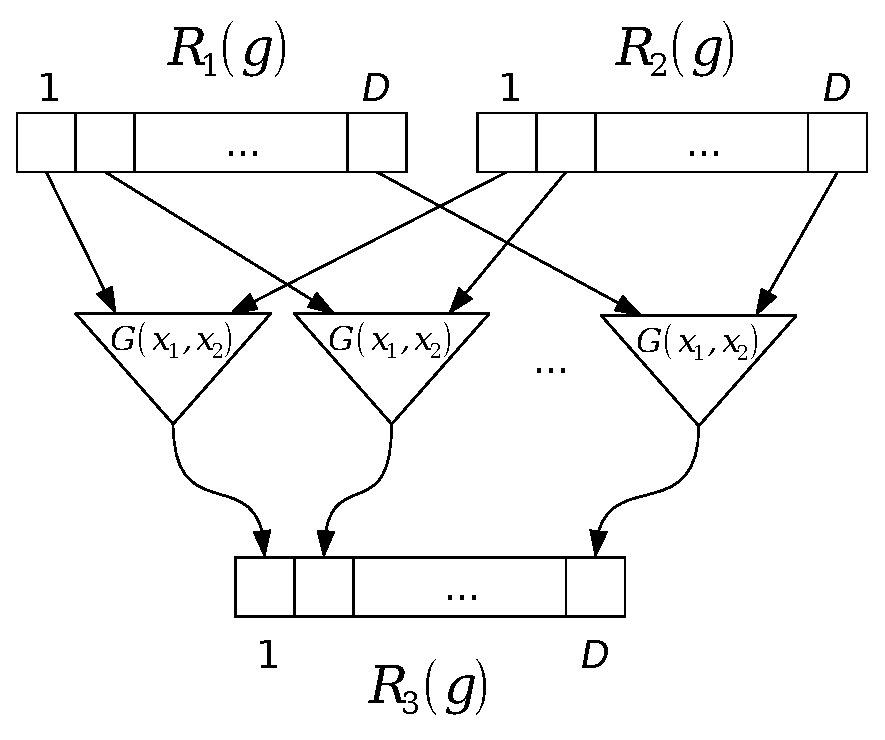
\includegraphics[width=7cm]{./bitslice.eps}
	\caption{Simultaneous computation of $D$ instances of the circuit $C(f)$ with bit-slicing technique} 
	\label{fig:bitsl} 
\end{figure}

We will call the process of computation of the function $f$ (represented by the circuit C$(f)$ with m inner nodes) 
on a single input from $\{0,1\}^n$ a \textit{thread}, by analogy with the computational threads 
in a SIMD device. Thus, with the use of bit-slicing technique, it takes $m$
instructions to execute $D$ threads.

Now we describe the details of bit-slicing implementation of the A5/1
generator. Suppose that a computational device is able to calculate $D$
instances of any function from the basis $B=\{\land,\lor,\neg,\oplus\}$. Each
of $n\in\{1,...,64\}$ cells of LFSR1-3 gets a corresponding word $W_n\in\{0,1\}^D$:

\begin{gather*}
	LFSR1:W_1,...,W_{19}; \\
	LFSR2:W_{20},...,W_{42}; \\
	LFSR3:W_{43},...,W_{64}.
\end{gather*}

In bit-slicing technique, the shifting of the LFSR register (LFSR1 in this
example) will take the following form: 
\begin{gather*} 
	W'_1=W_{19} \oplus W_{18} \oplus W_{17} \oplus W_{14}, \\
	W'_n=W_{n-1}, n \in \{2,...,19\},
\end{gather*}
where $\oplus$ is the bitwise addition modulo 2 of Boolean vectors of length
$D$ operator. The calculation of the keystream bit will look like:
\begin{gather*} 
	W_{out}=W_{19} \oplus W_{41} \oplus W_{64}.
\end{gather*}

The conditional clocking is somewhat more complex to implement in bit-slicing
technique. First, to know if the LFSRs should be shifted or not, one needs to
calculate the corresponding shifting flags $F_1,F_2,F_3$ using the majority
function: 
\begin{gather*} 
	W_{maj}=maj(W_9,W_{30},W_{52})=(W_9 \wedge W_{30}) \vee (W_9 \wedge W_{52}) \vee (W_{30} \vee W_{52}), \\
	F_1 = W_9 \oplus {\neg W_{maj}}, \\
	F_2 = W_{30} \oplus {\neg W_{maj}}, \\
	F_3 = W_{52} \oplus {\neg W_{maj}}.
\end{gather*} 
Here all operations are bitwise operations over vectors of the length $D$.

To implement the conditional shifting of an LFSR one can use the bitwise
counterpart of the \textit{bitselect} function of arity 3: 
\begin{gather*} a,b,c \in \{0,1\}; \\ BS(a,b,c) = \left\lbrace
	\begin{array}{ll} b,a=1, \\ c,a=0.
	\end{array} \right.
\end{gather*} 

If the computational architecture lacks the hardware implementation of this
function, it can be emulated with the usage of the standard bitwise functions
corresponding to the matching functions from the basis $B$:
\begin{gather*} BS(a,b,c) = (a \wedge b) \vee (\neg a \wedge c).
\end{gather*}

Shifting LFSR1 with the use of bitwise counterpart of $BS(a,b,c)$ and the corresponding shifting flag $F_1$
looks the following way (example for LFSR1):
\begin{gather*} 
	W'_1 = BS(F_1, (W_{19} \oplus W_{18} \oplus W_{17} \oplus W_{14}), W_1);
	\\W'_n = BS( F_1, W_{n-1}, W_n), n \in \{2,..,19\}.
\end{gather*}

Some important details about bit-slicing implementation of the Anderson's
attack should still be covered. Anderson's attack follows 2 steps:
\begin{enumerate} 
	\item Calculation of the values of 11 bits of LFSR2 lying left of the
	 clocking bit using the information from the guessed 53 bits and
	 the known keystream.
	\item Clocking the generator as normal to check if the guessed filling of
	 the generator matches the known keystream.
\end{enumerate}

The irregular clocking of the A5/1 generator makes it generally impossible to
predict how many clockings of the generator (bits of keystream) would be
needed to shift 11 times LFSR2 to complete Stage 1 of the attack.
Therefore, we again put to use the bitselect function to implement the split of
the attack into 2 stages. Each individual thread should be able to advance from Stage 1 to Stage 2 
independently of other threads. To achieve this, we introduce the special 
Boolean vector $\phi = (\phi_1,...,\phi_D)$, called
\textit{attack stage flag}. The thread with number $i, i \in \{1,...,D\}$ being in
Stage 1 of the attack corresponds to $\phi_i = 0$, and Stage 2 of the
attack corresponds to $\phi_i=1$. Let $y_1,...,y_{64}$ be the bits of the
keystream analyzed. Now the shifting of LFSR2 takes into account the stage of the
attack through the usage of the attack stage flag: 
\begin{gather*} 
	W^\ast_{41} = BS(\phi, W_{41},(y \oplus W_{19} \oplus W_{64}));\\
	W'_{20} = BS(F_2,(W^\ast_{41} \oplus W_{40}), W_{20});\\
	W'_n = BS(F_2,W_{n-1},W_n), n \in \{21,...,41\}. 
\end{gather*}

Here $W^\ast_{41}$ is a helper vector holding temporary data, $y$ is the
current bit of the keystream, in the form of a vector consisting of $D$ copies
of the corresponding bit of the keystream. The goal of Stage 1 is to
calculate the last bit of LFSR2 from known keystream bits and 
guessed last bits of LFSR1 and LFSR3. At Stage 2 the last bit of
LFSR2 is known and the generator is clocked as normal. For the
$i$-th thread the attack stage flag $\phi_i$ is set to 1 after LFSR2 of this thread 
was shifted 11 times. To count the number of LFSR2 shifts individually for each thread, 
bit-slicing implementation of an incremental counter is used.

Anderson's attack described above was implemented on an NVIDIA GPU
with the use of CUDA SDK 8.0 \cite{CudaSdk8}. The comparison of the performance of
a GPU to a CPU in execution of bit-slicing and LFSR precomputation-based
\cite{DBLP:conf/fse/BiryukovSW00} implementations of Anderson's attack is shown in
\Cref{tab:gpuspeed}. In the third implementation LOP3.LUT\footnote{LOP3.LUT is a special instruction that implements
arbitrary bitwise arity 3 functions in hardware.} instruction was used as a substitute
for the bitselect instruction.

\begin{table} 
	\caption{Performance of two implementations of
	Anderson's attack (search space size is $2^{53}$) on a CPU and a GPU, measured
	in millions of key checks per second.} 
	\label{tab:gpuspeed}
	\begin {center} 
	\begin{tabular} {| l | l | l |} 
	\hline Computational device & Bit-slicing &
		LFSR precomputation \\ 
		\hline
		\hline CPU Intel Core I7 930 & 37 & 7
		\\ 
		\hline GPU NVIDIA GTX 1050 Ti & 9180 & 483 \\ 
		\hline GPU NVIDIA GTX
		1050 Ti (LOP3.LUT) & 11950 & - \\ \hline
	\end{tabular}
\end {center}
\end{table}

Data provided in \Cref{tab:gpuspeed} tells us that even one mid-range
consumer GPU is enough to make Anderson's attack runtime practical (it
will take around 250 hours). A modern computational cluster outfitted with GPUs
will perform the attack in mere minutes. Anderson's attack's
advantage over the rainbow-tables attack \cite{Nohl2010} is the former's ability
to restore the secret key from 64 bits of keystream with the 100\% probability.
Its advantge over the attack described in \cite{DBLP:conf/ches/GendrullisNR08} is in a usage of a
consumer-grade off-the-shelf hardware.

\section{Implementation of Anderson's Attack in a volunteer computing
project}
\label{sec:boinc}

In order to solve 10 cryptanalysis problems for the A5/1 keystream generator we
launched the volunteer computing project AndersonAttack@home. The client (computing)
application of this project is based on the CUDA implementation, which was
described in the previous section.

Volunteer computing is a type of distributed computing which uses computational resources of PCs (hosts) of private persons called volunteers \cite{DBLP:conf/ccgrid/AndersonF06}. Each volunteer computing project is designed to solve one or several hard scientific problems. Each volunteer computing project consists of the following basic parts: server daemons, database, web site and client application. Daemons include \textsc{work generator} (it generates tasks to be processed), \textsc{validator} (it checks the correctness of the results received from volunteer PCs) and
\textsc{assimilator} (aimed at processing correct results). A client application should
have versions for the most widespread computing platforms. One of the attractive
features of volunteer computing is its low cost --- to maintain a project one
only needs a lightweight dedicated server working 24/7.

AndersonAttack@home is based on BOINC (Berkley Open Infrastructure for Network
Compuitng \cite{Anderson:2004:BSP:1032646.1033223}), which is the most popular platform for
volunteer computing. Each BOINC-based project is independent, but any user can take part in it 
with the help of the standard BOINC manager. This manager allows users to tune projects priorities and to
regulate the mode of PC usage. 

In order to increase the reliability of computations, BOINC uses a form of redundancy.
In particular, several (at least 2) identical tasks are created for each workunit. These tasks are processed
on different hosts, the results are compared on the project server by validator,
and are accepted only when a consensus is reached (the sufficient number of
successful results is called a \textit{quorum}). If tasks results for a particular workunit do not match, 
then the new copies of the task are created and scheduled for processing. The scheme of
a BOINC-based project with the quorum of 2 is shown on \cref{fig:boinc}.

\begin{figure}
	\centering
	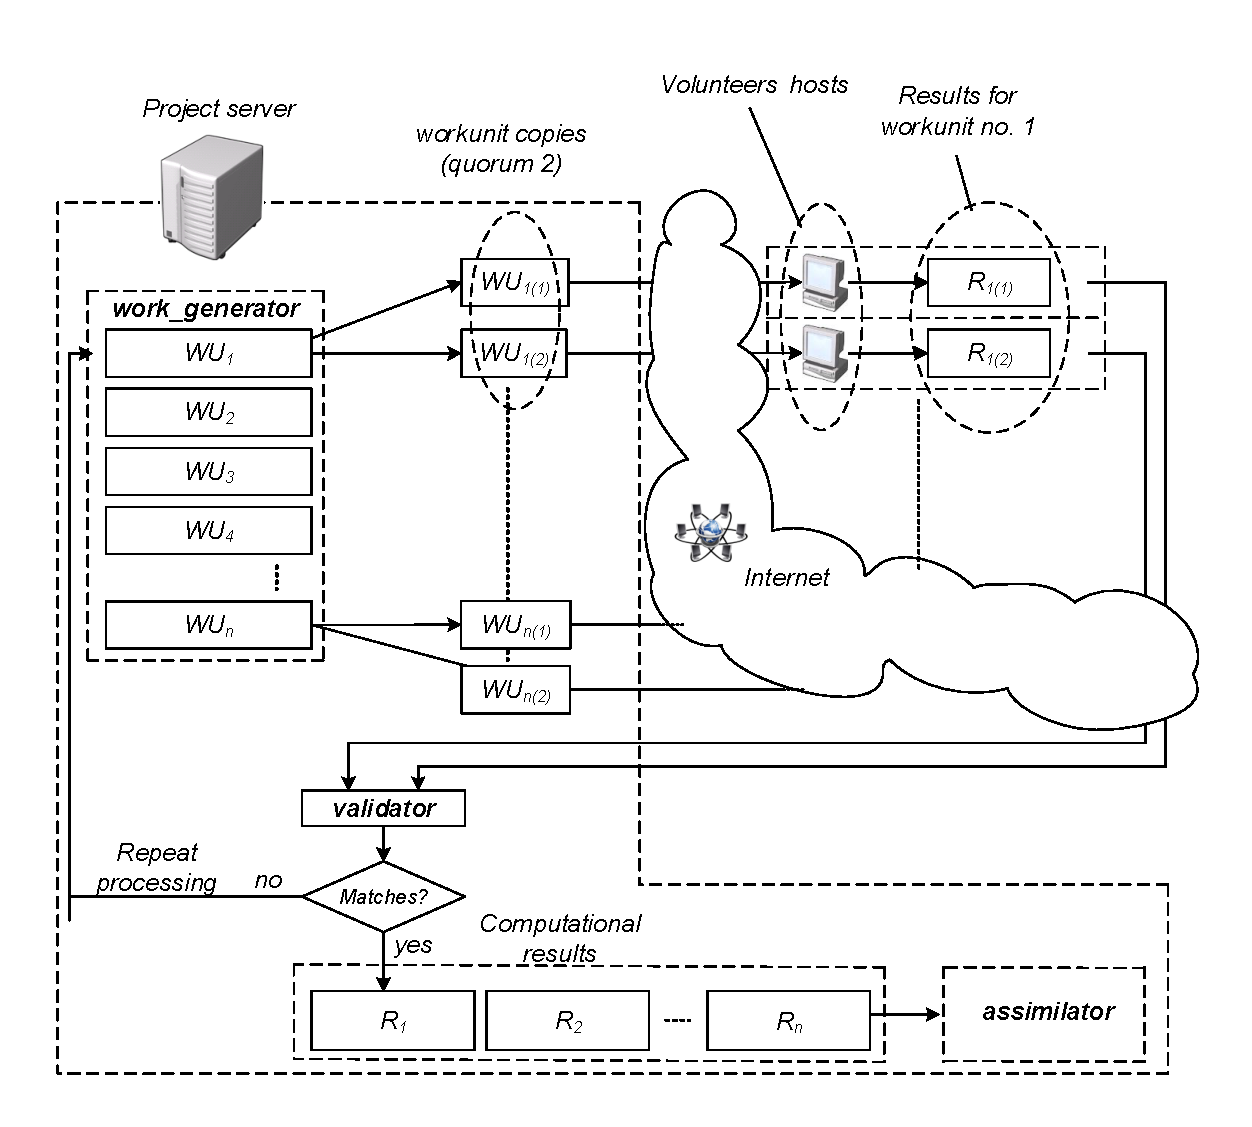
\includegraphics[width=10.5cm]{./BOINC_project_scheme.eps}
	\caption{The scheme of a BOINC-based project with the quorum of 2} 
	\label{fig:boinc} 
\end{figure}

In the first stage of our experiment, a family of workunits was generated on 
the project server. In each workunit values of 12 out of 53 guessing bits (see \cref{fig:a51and}) were fixed. Thus, 40960 workunits were generated for 10 cryptanalysis problems in total. Usually, the value of deadline for workunits in BOINC projects is 10-14 days. In
our project, we used a deadline of 1 day, because the experiment was quite
small. In the next stage, all generated workunits were processed in a desktop
grid formed by the project's hosts. This took about 7 days. As a result, solutions
for all considered problems were successfully found (see \Cref{tab:keys}). It should be noted, 
that for 7 out of 10 problems the collisions were found.

\begin{table} 
\caption{} 
\label{tab:keys} Original secret keys and collisions of the
	generator A5/1 (in hexadecimal format).
	\begin {center} 
		\begin{tabular}
			{| l | l | l | l |}
			\hline
			Instance & Keystream & \multicolumn{2}{|l|}{Secret key} \\ 
			\hline
			\hline
			1 & 0x770c0410869366f1 & original & 0x11b8e4340276c4ee \\
			  &                    & collision & 0x42634f3266d302a3 \\ 
			\hline
			2 & 0xae9590560c26e9ed & original & 0x4c656fd73e59ab9b \\
			  &                    & collision & 0xcf23e4722e3cfb68 \\ 
			\hline
			3 & 0xdd4b3ab7f6cf8224 & original & 0x09429d158555f4b3 \\
			  &                    & collision & 0x09429d158553e967 \\
			  &                    & collision & 0x40e5f2c8128a1781 \\ 
			\hline
			4 & 0x93cd42d97eb75fd9 & original & 0xfa386a338355aafd \\
			  &                    & collision & 0xf9e81096bb4d0aad \\ 
			  &                    & collision & 0xf9e81096bb4a8556 \\ 
			\hline
			5 & 0x925e423c98121152 & original & 0xe5cf81035ce5fbe2 \\ 
			\hline
			6 & 0x3b3464bd6e377b87 & original & 0x9625e9d810b46248 \\
			  &                    & collision & 0xf5aa1be2d6c36e18 \\ 
			  \hline
			7 & 0x0367d29121dd1677 & original & 0xd1b8b06086edf162 \\ 
			\hline
			8 & 0x6b49230b7fc0249d & original & 0xbe81a896968c486b \\ 
			\hline
			9 & 0xc65847556752d14c & original & 0xb6f65d2855a211c0 \\ 
			  &                    & collision & 0xb6f65d2855a508e0 \\ 
			\hline
			10& 0x07bb7f83d26072ec & original & 0x122a1a2955286b9f \\ 
			  &                    & collision & 0xd5151aaa50490012 \\ 
			\hline
		\end{tabular}
	\end {center}
\end{table}

In the considered experiment the project's performance was comparable to that of a computational cluster equipped with 30 modern GPUs.
According to the BOINC statistics, 143 active hosts belonging to 90 volunteers participated in the experiment. Here by \textit{active host} we mean a host which correctly processed at least one task. Active volunteer has at least one active host.

\section{Related work}
\label{sec:related}

As was noted before, at the time of writing of our article the A5/1 algorithm
remains one of the most popular research objects among cryptography
specialists, along with DES and RSA algorithms. The exact authorship of this
algorithm is unknown, but some experts argue that chances are high that its
development should be attributed to a French special agencies. Numerous sources
describe the events that led to its structure leaking to general public. In
fact, its internal workings were already known to research community in 1994:
R. Anderson's note (a mailing list message) written in that period was one of
the first works on the A5/1 cryptanalysis. The complete knowledge of A5/1 was
acquired in 1999 as a result of the reverse engineering of a mobile phone.

Earlier we have mentioned Anderson's attack, which was the first attack on A5/1 with compexity less
than that of a trivial brute-force-based search over the whole keyspace. Shortly
afterwards J. Golic suggested the attack on ``Alleged'' A5/1, based on
linearization of the equations describing A5/1 \cite{Golic1997}. The Golic's attack
estimated complexity is $C \cdot 2^{40}$, where $C$ denotes the complexity of
solving a system of linear equations of quite large dimension over $GF(2)$. The next widely known attack on the A5/1 was presented in \cite{DBLP:conf/fse/BiryukovSW00}. To speed up the A5/1 generator the authors of that paper used the technique of precomputation of LFSRs we mentioned in \Cref{sec:bitslc}. It should be noted, that the attack presented in \cite{DBLP:conf/fse/BiryukovSW00}, along with those presented in
\cite{Biham2000,DBLP:journals/tit/EkdahlJ03,Barkan2008}, requires substantial
length of known keystream (at least several seconds). These attacks can be
considered realistic ones, but they do not demonstrate vulnerability of the GSM
protocol as evidently, as those belonging to the ``advanced brute force'' class,
that we will discuss below. For the rest of the section we consider an attack
to be practical, if its implementation is able to persistently find the
secret key by analyzing no more than 2 frames (912 bits) of a keystream. 
A keystream fragment of this length could always be extracted from the technical messages used during a call in a GSM network by exploiting the protocol vulnerability described in \Cref{sec:alg}.

It seems that the first practical attack was presented in \cite{DBLP:conf/ches/GendrullisNR08}. Its authors implemented the optimized variant of Anderson's attack on a specialized computational device of their
own design, assembled from 120 ``Xilinx Spartan 3'' FPGAs. They state that the attack took about 6 hours. It is worth
mentioning, that the COPACOBANA architecture was used to analyze several other ciphers, e.g. DES \cite{Guneysu2008}.

The first estimates of the time required for the cryptanalysis of A5/1 on a
computational cluster in the form of Boolean satisfiability problem (SAT \cite{DBLP:series/faia/2009-185})
were presented in \cite{PACO-2008}. The SAT-based cryptanalysis is
a perspective direction of cryptanalysis that seems to be on the rise for the last decade. It operates within the paradigm that the cryptanalysis problem can be efficiently represented in the form of a SAT
problem. This could be achieved with the help of special translators, such as
\cite{DBLP:conf/csiirw/ErkokM09,journals/lmcs/predrag,DBLP:conf/ecai/OtpuschennikovS16}. After the problem was translated
to SAT, it can be solved by state-of-the-art SAT algorithms which can
be launched in a distributed computing environment. The cryptanalysis time of A5/1
estimated in \cite{PACO-2008} was realistic, but since the exclusive usage of
the whole computational cluster for prolonged period of time was not an option at that moment,
the actual attack was performed a year later in a specialized grid-system
\cite{Posypkin2009}. In the following years these results were improved --- the
search space of $2^{31}$ SAT instances was processed completely and collisions
(different secret keys generating the same keystream) have been found
\cite{DBLP:conf/pact/SemenovZBP11}. At the same period it became apparent that 
this kind of cryptographic attack fits well into the ideology
of volunteer computing \cite{DBLP:conf/ccgrid/AndersonF06}. To bring this line of
thought to life in 2012 SAT@home \cite{Semenov2016} volunteer computing project
was launched. Through 4 years of its activity a number of hard combinatorial
problems were solved within the SAT paradigm. Among those were several dozens
cryptanalysis problems for the A5/1 generator (only one burst --- 114 bits of
keystream --- was used each time). These results were published in
\cite{DBLP:conf/pact/SemenovZ15,Semenov2016}.

The work \cite{Guneysu2008} included the estimates of time and disk space
required to create the rainbow-tables that would make it possible to
``break'' A5/1 on an average PC in several minutes. \cite{Guneysu2008} estimated
that these tables will require about 7 Tb of disk space. The A5/1 Cracking Project put the
significantly more compact (2 Tb) tables into public domain at the end of 2009
\cite{Nohl2010}. By analyzing 2 frames (912 bits) of known keystream with
the help of these tables one can restore the secret key with probability of
success over 85\%. This method of cryptanalysis of the A5/1 algorithm could be
assumed to be the most practical one. The fact that it does not provide 100\%
guarantee of success does not matter in real circumstances. It should be noted that if the tables are lost, it will require a
vast amount of computational resources to generate them again.

Finally, the attack we presented in this paper does not lose on the practical
side to the rainbow-tables attack, because it allows to perform the
cryptanalysis with 100\% success rate in a period of several hours in a small
volunteer computation project. Moreover, the attack requires only 64 bits of
known keystream. Volunteer computing is rising in popularity and
publicity in the last years, so any attractive problem (like a cryptanalysis of one
of the most widely used ciphers) immediately gets volunteers attention.

\section{Conclusion}
\label{concl}
In the present paper, we made a GPU-based implementation of Anderson's attack on the A5/1 keystream generator. The meticulous adaptation of this attack to the SIMD architecture made it possible to solve several cryptanalysis problems in a BOINC-based desktop grid.

We would like to express the hope that the efficiency of our implementation of the attack will serve as yet another strong argument against the usage of the A5/1 algorithm in the transfer of sensible data through GSM networks.

\section*{Acknowledgment}
The research was funded by Russian Science Foundation (project No. 16-11-10046). The authors would like to thank Stepan Kochemazov for helpful discussions and valuable comments.

\bibliographystyle{splncs03}
\bibliography{pact2017_bulavintsev_ref}

\end{document}
